\documentclass{beamer}
\usepackage[french]{babel}
\usepackage{inputenc}
\usetheme{metropolis}
\usecolortheme{cormorant}
\usepackage{minted}
\usepackage {ifthen}
\newboolean{printCode}
\setboolean{printCode}{true}
% \usemintedstyle{trac}
\usepackage{xcolor}
\usepackage{hyperref}
\usepackage{graphicx}
\usepackage{ulem}  % texte barré

% texte surligné
\usepackage{soul}
\usepackage{color}
\newcommand{\hilight}[1]{\colorbox{lightgray}{#1}}

\title{Technique et chaîne de publication électronique avec XSLT}
\date{2023, 9 janv. - 13 fev.}
\author{Jean-Damien Généro}
\institute{École nationale des chartes -- M2 TNAH}

\begin{document}

  \maketitle
  
  \begin{frame}{Contact}
  \Large
      \begin{itemize}
          \item \textbf{jean-damien.genero@cnrs.fr}
      \end{itemize}
  \end{frame}


    \begin{frame}{Objectifs}
  \Large
      \begin{itemize}
          \item \textbf{XPath}
          \begin{itemize}
              \item Naviguer dans un arbre XML
              \item Manipuler les principales fonctions XPath
          \end{itemize}
          \item \textbf{XSLT}
          \begin{itemize}
              \item Manipuler les règles (\textit{templates}) basiques
              \item Manipuler les conditions et les boucles
          \end{itemize}
          \item \textbf{Édition numérique}
          \begin{itemize}
              \item Transformer un document XML en un autre document XML
              \item Transformer un document XML en un document HTML
              \item Transformer un document XML en un document \LaTeX
          \end{itemize}
      \end{itemize}
  \end{frame}
   

  \section{Écosystème XML}
  \begin{frame}{Écosystème XML/ Principes généraux}
  \Large
  \begin{itemize}
      \item \textbf{XML $\rightarrow$} \textit{langage de balisage qui encode une description de la mise en page et de la structure logique d'un document}
      \begin{itemize}
          \item \textbf{XPath $\rightarrow$} \textit{langage de requête pour naviguer dans la structure hiérarchique d'un document XML à l'aide de chemins} ;
      \end{itemize}
      \bigskip
      \item \textbf{XSL $\rightarrow$} \textit{spécifications pour la transformation de doc XML à l'aide de feuilles de style} ;
      % \begin{itemize}
          % \item Feuille de style (\textit{stylesheet}) $\rightarrow$ \textit{exprime des intentions sur la manière dont un contenu structuré [i. e. un doc XML] doit être présenté} ;
      % \end{itemize}
      \bigskip
      \item \textbf{XSLT $\rightarrow$} \textit{un langage conçu pour transformer des documents XML en d'autres documents selon les spécifications XSL}.
  \end{itemize}
   
   \footnotesize W3C Recommendations : \href{https://www.w3.org/TR/xml11/}{XML}, \href{https://www.w3.org/TR/xpath-31/}{XPath}, \href{https://www.w3.org/TR/xsl/}{XSL}, \href{https://www.w3.org/TR/xslt-30/}{XSLT}.
   
  \end{frame}
  
  \begin{frame}{Écosystème XML/ Schéma}
      \begin{center}
          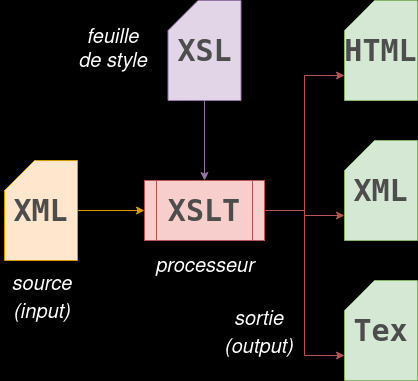
\includegraphics[width=8cm, height=7cm]{img/ecosysteme_xml.jpeg}
      \end{center}
  \end{frame}
  
  \begin{frame}{Écosystème XML/ Navigation XPath et de règles XSL}
  \Large
  \begin{itemize}
      \item \textbf{Navigation XPath} :
      \begin{itemize}
          \item Doc XML = structuré, on parle d'\og \textbf{arbre} \fg{} (\textit{XML tree}) ; 
          \item \textbf{Itinéraire} vers une balise (\og \textbf{parent} \fg{} $\rightarrow$ \og \textbf{enfant} \fg{}) ; % comparable au chemin dans une arborescence de fichiers avec la commande cd + sens ascendant et descendant ;
          \item Rédaction dans une \textbf{syntaxe propre}. % (langage intégré)
      \end{itemize}
      \bigskip
      \item \textbf{Règle XSL (\textit{template})} :
      \begin{itemize}
          \item \textbf{Agir} sur une ou plusieurs balises (\textit{transform}) ;
          \item Exemples : \textbf{copier} balise + contenu, copier uniquement le contenu et l'\textbf{insérer} dans une nouvelle balise, \textbf{ajouter} ou \textbf{supprimer} un attribut, etc. ;
          \item Rédaction dans une \textbf{syntaxe XML} (langage à balises).
      \end{itemize}
      \bigskip
      \item \textbf{Utilisation avec d'autres langages}
      
      \normalsize (\texttt{Python} :  \texttt{lxml}).
  \end{itemize}
   
  \end{frame}
  
\begin{frame}[fragile]
\frametitle{Écosystème XML/ Exemple d'un chemin XPath}
% définir le concept de "navigation dans un arbre xml" (passe par les balises)
% Soit un arbre XML (\textit{XML tree}) :
\begin{itemize}
    \item Comment accéder aux balises \texttt{<p>} avec XPath ?
\end{itemize}
\small
\begin{minted}{xml}
    <TEI>
        <teiHeader/>
        <text>
            <body>
                <p>title</p>
                <p>text</p>
            </body>
        </text>
    </TEI>
\end{minted}
\normalsize
\begin{itemize}
          \item \texttt{<TEI>} $\rightarrow$ \texttt{<text>} $\rightarrow$ \texttt{<body>} $\rightarrow$ \texttt{<p>}
          \item Traduction XPath : \texttt{/TEI/text/body/p}
          \begin{itemize}
              \item Simplification : \texttt{//body/p} (\texttt{/\sout{TEI/text}/body/p})
          \end{itemize}
      \end{itemize}
\end{frame}
  
    \begin{frame}[fragile]
   \frametitle{Écosystème XML/ Exemple d'une règle XSL}
        \begin{itemize}
            \item Comment appliquer une règle XSL aux balises \texttt{<p>} ?
            \begin{itemize}
                \item Une règle XSL est toujours contenue dans une balise \texttt{<xsl:template/>} possédant un \texttt{@match}.
            \end{itemize}
            \item Indiquer le chemin XPath vers les \texttt{<p>} dans  l'\texttt{@match}.
        \end{itemize}
        \bigskip
        \begin{minted}{xslt}
        <xsl:template match="/TEI/text/body/p">
            <xsl:copy-of select="."/>
        </xsl:template>
        \end{minted}
        ou
        \begin{minted}{xslt}
        <xsl:template match="//body/p">
            <xsl:copy-of select="."/>
        </xsl:template>
        \end{minted}
   \end{frame}

    \section{XPath}
    
    \begin{frame}{XPath/ Syntaxe}
        \Large
        \begin{itemize}
            \item \textbf{N\oe ud} (\textit{node}) = un composant de l'arbre XML. Sept types, dont : \textbf{balise}, \textbf{attribut}, \textbf{\textit{text}}, \textit{namespace}.
            %% Peut être inclus dans un chemin XPath. 7 noeuds : https://www.w3schools.com/xml/xpath_nodes.asp
            \bigskip
            \item Écrire un chemin (\textit{expression}) : succession de n\oe uds séparés par l'\textbf{opérateur /} ;
            \begin{itemize}
            \Large
                \item \texttt{/TEI/text/body/p}
            \end{itemize}
            \bigskip
            \item Axe (direction) basique : \textbf{parent $\rightarrow$ enfant}
        \end{itemize}
        
    \end{frame}

        \begin{frame}{XPath/ Axes de relation}
        \Large
        \begin{itemize}
            \item Un axe permet de qualifier la \textbf{relation} entre le \textbf{n\oe ud de contexte} et un ou des \textbf{autre(s) n\oe ud(s)}.

            \bigskip

            \item 13 axes XPath, dont :
            \begin{itemize}
            \large
                \item \texttt{parent::} $\rightarrow$ n\oe ud immédiatement au-dessus ;
                \item \texttt{child::} $\rightarrow$ n\oe ud immédiatement en-dessous ;
                \item \texttt{following-sibling::} $\rightarrow$ n\oe ud(s) après celui de contexte et qui ne fait/font pas partie de ses descendants ;
                \item \texttt{ancestor}, \texttt{descendant}, \texttt{preceding}, etc.
                %% https://developer.mozilla.org/fr/docs/Web/XPath/Axes
                %% https://spip.teluq.ca/inf6450/spip.php?article111
                %% https://svground.fr/xpath-axes.php#following-sibling
                %% preceding-sibling : que les noeuds de même niveau
                %% folloxing : les noeuds de même niveau + leurs descendants
            \end{itemize}
        \end{itemize}
        
    \end{frame}

    \begin{frame}{XPath/ Axe \texttt{ancestor::}}
        \begin{center}
            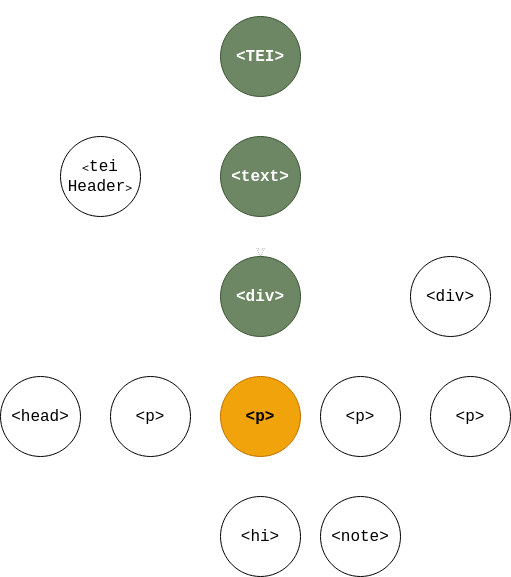
\includegraphics[width=7cm]{img/ancestor.png}
        \end{center}
    \end{frame}

    \begin{frame}{XPath/ Axe \texttt{child::}}
        \begin{center}
            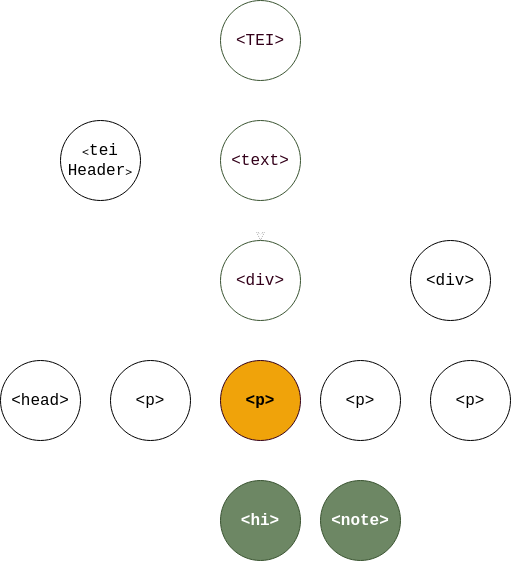
\includegraphics[width=7cm]{img/xslt_child.png}
        \end{center}
    \end{frame}

    \begin{frame}{XPath/ Axe \texttt{following-sibling::}}
        \begin{center}
            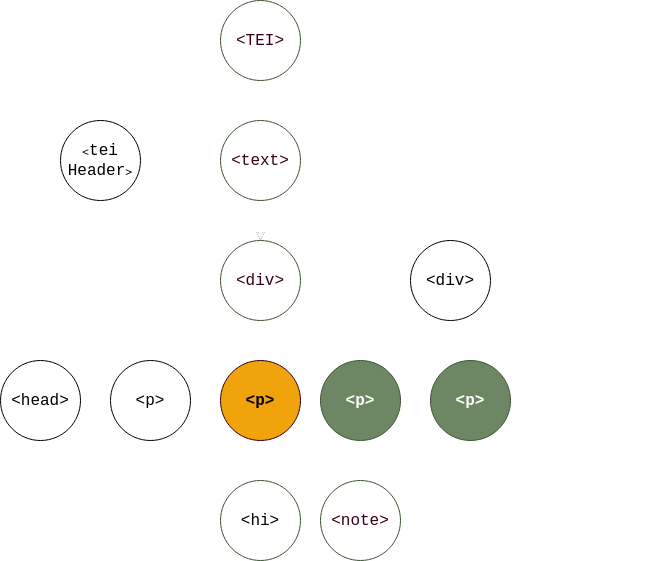
\includegraphics[width=9cm]{img/xslt_following_sibling.png}
        \end{center}
    \end{frame}

    \begin{frame}{XPath/ Abbréviations des axes}
    \Large
        \begin{itemize}
            \item (Racine $\rightarrow$ \textbf{/})
            \item \texttt{self::} $\rightarrow$ \textbf{.} \textit{(n\oe ud courant)}
            \item \texttt{attribute::} $\rightarrow$ \textbf{@}
            \bigskip
            \item Donc : vous pouvez écrire \texttt{//div/@n} au lieu de \texttt{//div/attribute::n}.
        \end{itemize}
    \end{frame}
    
    \begin{frame}{XPath/ Prédicats : définition}
        \Large
        \begin{itemize}
            \item Prédicat (filtre) = \textbf{condition} qui doit être satisfaite par le n\oe ud courant (existence d'un attribut, valeur d'un attribut, position d'une balise, etc.).
            \item Écrit entre crochets \texttt{[ ]}.
            \bigskip
            \item \texttt{//div[@n='2']/head} = le \texttt{<head>} de la \texttt{<div>} avec un \texttt{@n} de valeur \texttt{2}.
            \bigskip
            \item \texttt{//body/div[@n='2']/p[2]} = \textbf{?}
        \end{itemize}
    \end{frame}

    \begin{frame}{XPath/ Prédicats : exemples}
        \Large
        \begin{itemize}
            \item \texttt{//tag[position()=1]} ou \texttt{//tag[2]} $\rightarrow$ condition de position (\texttt{<tag>} n°2) ;
            \bigskip
            \item \texttt{//tag[last()]} $\rightarrow$ dernier \texttt{<tag>} ;
            \bigskip
            \item \texttt{//tag[@foo='bar']} $\rightarrow$ expression logique (\texttt{<tag>} avec un \texttt{@foo} dont la valeur est \texttt{bar}) ;
        \end{itemize}
    \end{frame}

    \begin{frame}{XPath/ Notions essentielles}
        \Large
        \begin{itemize}
            \item Arbre XML, racine, n\oe uds (7) ;
            \item Chemin XPath, opérateur / ;
            \item Axes de relation (13) ;
            \item Prédicats.
        \end{itemize}
    \end{frame}

    \begin{frame}{XPath/ Exercice. \textit{Saint Julien l'hospitalier}.}
        \Large
        \begin{itemize}
            \item Donner le chemin de la racine vers \texttt{<author>} dans le \texttt{<sourceDesc>}.
            \bigskip
            \item Utiliser un prédicat pour sélectionner les \texttt{<title>} ayant pour texte \texttt{Trois Comtes}.
        \end{itemize}
    \end{frame}

    \section{XSLT : élément racine et instructions de premier niveau}

    \begin{frame}{XSLT/ Définition}
        \Large
        \begin{itemize}
            \item XSLT $\rightarrow$ un \textbf{langage de programmation déclaratif} ;
            \item Permet de \textbf{transformer un doc XML} en un autre doc  (\texttt{.xml}, \texttt{.html}, \texttt{.tex}, etc.) ;
            \item Transformation opérée par un \textbf{processeur XSLT}
            \begin{itemize}
                \item \textbf{Construit} l'arbre output, \textbf{transforme} l'arbre input et \textbf{sérialise} le document output ;
                % sérialisation = processus de génération du document de sortie selon les spécifications données (= templates xslt)
                % https://www.w3.org/TR/xslt-xquery-serialization-31/
                \item Le plus connu $\rightarrow$ \textbf{Saxon} (en ligne de commande) ;
                \item Généralement \textbf{intégré} à des logiciels (\textbf{Oxygen}) ou des librairies (\textbf{python : lxml}).
            \end{itemize}
        \end{itemize}
    \end{frame}

    \begin{frame}{XSLT/ La feuille de style}
    \Large
        \begin{itemize}
            \item Feuille de style XSL == un doc XML \texttt{.xsl} ;
            \item Contient des instructions ou règles (\textit{templates})  ;
            \item Élément racine : \texttt{<xsl:stylesheet>}
            % balises xsl commencent toujours par xsl: pour ne pas les confondre avec des balises d'autres langages (notamment celui de l'output)
        \end{itemize}
        \bigskip
        \bigskip
        \begin{itemize}
            \item \textbf{Dans Oxygen $\rightarrow$ ouvrir un nouveau doc \og XSLT Stylesheet \fg.}
            \item \textbf{Observer les attributs de l'élément racine.}
        \end{itemize}
    \end{frame}

    \begin{frame}{XSLT/ Élément racine : \texttt{<xsl:stylesheet>} (1/2)}
    \Large
    Attributs présents de base dans Oxygen :
        \begin{itemize}
            \item \texttt{@xmlns:xsl} : espace de nom (\textit{namespace}) XSL ;
            \item \texttt{@xmlns:xs} : espace de nom XML ;
            \item \texttt{@xmlns:tei} : espace de nom TEI ;
            \item \textbf{!} \texttt{@exclude-result-prefixes} : liste des préfixes qui ne seront pas copiés dans l'output (\texttt{xs}, \textit{à ajouter :} \texttt{tei}) ;
            \item \texttt{@version} : version de XSL (1, 2 ou 3).
        \end{itemize}
    \end{frame}

    \begin{frame}{XSLT/ Élément racine : \texttt{<xsl:stylesheet>} (2/2)}
    \Large
    Attributs à ajouter dans Oxygen :
    \bigskip
        \begin{itemize}
            \item \texttt{@xmlns} : espace de nom de l'élément racine de l'output ;
            \begin{itemize}
            \large
                \item évite l'ajout de cet espace de nom sur chaque élément "matché" par une règle (contenu dans le \texttt{@match} de \texttt{<xsl:template>}).
            \end{itemize}
            \bigskip
            \item \texttt{@xpath-default-namespace} :  espace de nom des chemins XPath.
            \begin{itemize}
            \large
                \item évite de devoir écrire le préfix \texttt{tei:} devant chaque n\oe ud d'une expression XPath.
            \end{itemize}
        \end{itemize}
    \end{frame}

    \begin{frame}[fragile]{XSLT/ Instruction de 1\up{er} niveau : \texttt{<xsl:output>}}
    \Large
        \begin{itemize}
            \item Instruction de premier niveau ;
            \item \og \textbf{contrôle les caractéristiques du document de sortie} \fg.
        \end{itemize}

        \begin{minted}{xml}
<xsl:output
    method="xml | html | text"
    indent="yes | no"
    omit-xml-declaration="yes | no"
    encoding="UTF-8"
/>
        \end{minted}
    \end{frame}

    \begin{frame}[fragile]{XSLT/ Écriture d'une règle : \texttt{<xsl:template>} (1/3)}
        \Large
        \begin{itemize}
            \item \texttt{<xsl:template>} $\rightarrow$ définir une règle ;
            \bigskip
            \item Possède un \texttt{@match} avec pour valeur un chemin XPath qui donne l'emplacement du n\oe ud sur lequel sera appliquée la règle.
            \bigskip
            \item Appliquer une règle vide en sélectionnant la racine :
        \end{itemize}

        \begin{minted}{xslt}
    <xsl:template match="/">
    </xsl:template>
        \end{minted}
        % deux constats : pas d'erreur (la transformation a lieu) + il ne se passe rien, le doc output est vide.
        % conclusion : une règle vide ne copie rien, utile si je ne veux pas qu'un élément de l'input pour l'output
    \end{frame}

    \begin{frame}[fragile]{XSLT/ Écriture d'une règle : \texttt{<xsl:template>} (2/3)}
        \Large
        \begin{itemize}
            \item Appliquer la règle \texttt{copy-of} sur la racine :
        \end{itemize}

        \begin{minted}{xslt}
    <xsl:template match="/">
        <xsl:copy-of select="."/>
    </xsl:template>
        \end{minted}
        % constats : doc input est copié sans modiffication
        % donc : copy-of >> copie de tout l'élément (balises, attributs, texte) dans le @select

        \begin{itemize}
            \item Comment copier le \texttt{<body>} dans l'output, mais sans le \texttt{<teiHeader>} ?
        \end{itemize}
    \end{frame}

    \begin{frame}[fragile]{XSLT/ Écriture d'une règle : \texttt{<xsl:template>} (3/3)}
    \Large
        \begin{itemize}
            \item Comment obtenir cet arbre en output ?
        \end{itemize}
        \normalsize
        \begin{minted}{xml}
    <div>
        <head>Trois comtes</head>
        <!-- copie de la div n°1 de l'input -->
        <div n="1">
            <head>I.</head>
            ...
        </div>
        <!-- copie de la div n°2 de l'input -->
        <div n="2">
            <head>II.</head>
            ...
        </div>
    </div>
        \end{minted}
        
    \end{frame}

    \begin{frame}{XSLT : première approche. Notions essentielles}
        \Large
        \begin{itemize}
            \item Transformation et feuille de style XSL ;
            \bigskip
            \item Manipulation de XSL avec Oxygen ;
            \bigskip
            \item Élément racine : \texttt{<xsl:stylesheet>} et ses attributs ;
            \bigskip
            \item Instructions de premier niveau :
            \begin{itemize}
            \Large
                \item \texttt{<xsl:output>} ;
                \item \texttt{<xsl:template>} et son \texttt{@match}.
            \end{itemize}
        \end{itemize}
    \end{frame}
\end{document}
